\subsection{Caso d'uso UC4: Salvataggio presentazione}
\begin{figure}[h] 
	\centering 
	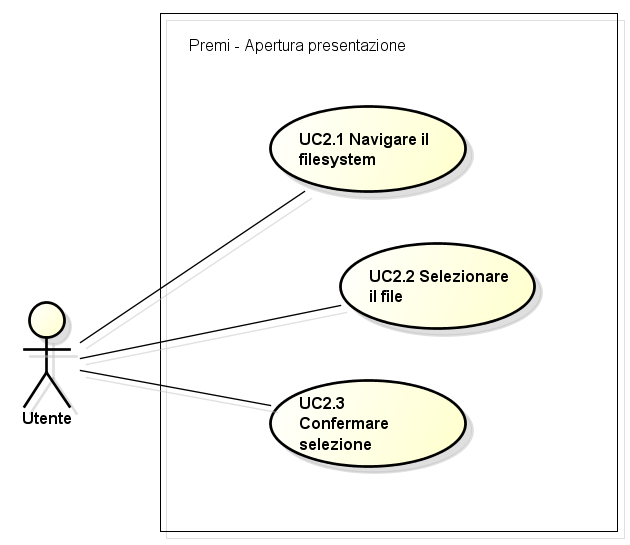
\includegraphics[scale=0.45] {img/UC4.png} 
	\caption{UC4 - Salvataggio presentazione} 
\end{figure}

\begin{itemize}
	\item \textbf{Attori:} Utente;
	\item \textbf{Scopo e descrizione:} L'utente ha creato una presentazione slide e vuole salvarla in una specifica cartella;
	\item \textbf{Precondizione:} Il sistema è in attesa che l'utente selezioni la funzione salva;
	\item \textbf{Flusso degli eventi:}
	\begin{enumerate}
		\item L'utente seleziona la funzione salva [UC4.1];
		\item L'utente seleziona la cartella nella quale salvare la presentazione [UC4.2];
		\item L'utente scrive il nome del file [UC4.3];
		\item L'utente può selezionare un file già esistente da sovrascrivere [UC4.4];
		\item L'utente conferma il salvataggio [UC4.5].
	\end{enumerate}
	\item \textbf{Postcondizione:} Il sistema salvato la pesentazione nella cartella selezionata con il nome indicato.
\end{itemize}

\subsection{Caso d'uso UC4.1: Selezionare funzione salva}
\begin{itemize}
	\item \textbf{Attori:} Utente;
	\item \textbf{Scopo e descrizione:} L'utente seleziona dall'apposito menù la funzione di salvataggio per salvare la presentazione;
	\item \textbf{Precondizione:} Il sistema è in attesa che l'utente selezioni la funzione salva;
	\item \textbf{Postcondizione:} Il sistema apre la finestra di dialogo per il salvataggio.
\end{itemize}

\subsection{Caso d'uso UC4.2: Navigazione nel filesystem}
\begin{itemize}
	\item \textbf{Attori:} Utente;
	\item \textbf{Scopo e descrizione:} L'utente naviga il \gls{filesystem} per selezionare posizione di salvataggio della presentazione;
	\item \textbf{Precondizione:} Il sistema è in attesa che l'utente selezioni una cartella;
	\item \textbf{Postcondizione:} Il sistema aggiorna il percorso con quello scelto dall'utente.
\end{itemize}

\subsection{Caso d'uso UC4.3: Scrittura nome file}
\begin{itemize}
	\item \textbf{Attori:} Utente;
	\item \textbf{Scopo e descrizione:} L'utente deve inserire un nome valido con il quale salvare la presentazione;
	\item \textbf{Precondizione:} Il sistema permette all'utente di selezionare il nome della presentazione da salvare;
	\item \textbf{Postcondizione:} È stato inserito un nome valido per la presentazione che l'utente desidera salvare.
\end{itemize}

\subsection{Caso d'uso UC4.4: Seleziona file già esistente}
\begin{itemize}
	\item \textbf{Attori:} Utente;
	\item \textbf{Scopo e descrizione:} L'utente può selezionare una presentazione già esistente da sovrascrivere con il salvataggio;
	\item \textbf{Precondizione:} Il sistema contiene già una presentazione con il nome che l'utente desidera utilizzare;
	\item \textbf{Postcondizione:} La presentazione già esistente è stata selezionata dall'utente.
\end{itemize}

\subsection{Caso d'uso UC4.5: Conferma salvataggio}
\begin{itemize}
	\item \textbf{Attori:} Utente;
	\item \textbf{Scopo e descrizione:} L'utente conferma il salvataggio della presentazione;
	\item \textbf{Precondizione:} Il sistema ha ricevuto la richiesta di salvataggio della presentazione;
	\item \textbf{Postcondizione:} Il sistema ha salvato la presentazione selezionata dall'utente.
\end{itemize}
\newpage